%% ------------------------------------------------------- %%
%% SMT-LIB 2.0                                             
%% ------------------------------------------------------- %%
\section{SMT-LIB 2.0}
\subsection{Titre}
Presenter ici les nouveautes SMT 2.0
Considere l'interaction entre les solveurs SMT et d'autres outils.
Le chapitre V definit un langage de script (commandes, reponses) pour echanger des informations avec les solveurs SMT.

\begin{figure}
\centering
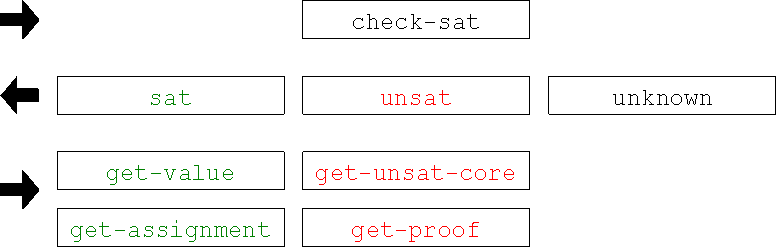
\includegraphics[scale=0.5]{SMT20.png}
\caption{SMT-LIB 2.0 Script Commands} 
\label{Fig:SMT-LIB 2.0}
\end{figure}

\subsection{Titre}
Interet.
\begin{itemize}
\item Information complementaire avec le livrable D7.
Le format des preuves retournees par get-proof n'est pas specifie dans SMT-LIB 2.0.
\item Information tres int�ressante pour l'integration dans Rodin.
\end{itemize}

\section{From Event-B to SMT-LIB 2.0}

\subsection{Titre}

\paragraph{}


\section{Targeted SMT solvers}
Voila un petit statut sur ce que j'ai pu observer sur les differents prouveurs SMT :
\begin{itemize}
\item CVC3. 
D'apres leur site, il supporte tous les formats SMT-LIB donc 2.0. 
Les logiques supportees (en tout cas celles presentees � la competition SMT 2010): $UFLRA$, $QF_UF$, $QF_RDL$, $QF_IDL$, $QF_BV$, $QF_UFIDL$, $QF_AX$, $AUFLIA+p$, $AUFLIA-p$, $AUFLIRA$, $QF_AUFLIA$, $QF_UFLRA$, $QF_UFLIA$, $QF_LRA$, $AUFNIRA$, $UFNIA$, $UFNIA+p$, $QF_LIA$, $QF_NIA$, $QF_UFNRA$, $QF_NRA$, $QF_ABV$.

\item CVC4. 
Prototype perdant beaucoup des fonctionnalites de CVC3 mais permettant d'avoir de meilleures perf sur la logique $QF_LRA$ de CVC3. Donc a mon avis pas tres interessant dans notre cas.

\item MathSAT 5. 
MathSat supporte a priori tout format SMT et possede des options permettant la generation de preuve et la recup�ration d'un  unsat core.
Logiques supportees (en tout cas celles presentees � la competition Smt 2010) : $QF_UF$, $QF_UFLRA$, $QF_UFLIA$, $QF_LRA$, $QF_LIA$.

\item MiniSmt. 
Supporte a priori tout format SMT.
Logiques supportees: $QF LIA$, $QF LRA$, $QF NIA$, $QF NR$. Celles presentees a la competition SMT 2010 sont les suivantes: $QF_NIA$, $QF_NRA$.

\item Open Smt. 
Arrive a parser des formats SMT-LIB 2.0 et possede options permettant la generation de preuve et recuperer un unsat core. Toutes les fonctionnalites SMT-LIB 2.0 ne sont pas encore supportees et une version prevue fin aout est censee etre plus stable.
Logiques supportees: $QF UF$, $QF IDL$, $QF RDL$, $QF LRA$, $QF UFIDL$ ( + $QF BV$, $QF AX$ et $QF UFLRA$ mais pas completement cf parser pas complet).

\item VeriT. 
Arrive a parser des formats SMT-LIB 2.0 mais ne supporte pas toutes les fonctionnalites SMT-LIB 2.0; il possede des options permettant la generation de preuve (pas de renseignements sur l'unsat core).
Logiques supportees (en tout cas celles presentees � la competition SMT 2010): $QF_UF$, $QF_RDL$, $QF_IDL$, $QF_UFIDL$.

\item Z3 (non presente � la competition). 
Supporte une partie de SMT-LIB 2.0 mais surement pas la globalite. Possede une option pour recuperer un unsat core et pour generer une preuve.
Attention, le get-unsat-core ne retourne pas necessairement les hypotheses telles qu'elles ont ete entrees. Celles-ci peuvent en effet avoir subi des transformations par le solveur.

\end{itemize}